% =============================================================================
%  Appendix A — Detailed Corpus Construction Pipeline
% =============================================================================

\section[\appendixname~\thesection]{Detailed Corpus Construction Pipeline}
\label{sec:appendix:corpus_pipeline}

This appendix contains the full procedural detail for the six stages of
corpus construction compressed in Section~\ref{sec:methodology:search} of the
main text. All record counts, tables, and figures reported here are the same
data summarised there; the appendix provides the complete walkthrough for
reproducibility and audit purposes.

\subsection*{A.1 Pre-Validated Corpora (G1--G6)}

In parallel with snowballing, six thematically focused pre-validated corpora
(Groups G1--G6) were assembled through targeted curation of leading
publication venues. Undermind, an AI-assisted academic search tool, was used
to accelerate retrieval of candidate papers from ACL, EMNLP, NeurIPS, ICML,
MLSys, and related venues for each of the six groups. The Undermind queries
are reproduced verbatim in Appendix~B. All inclusion decisions remained with
the human reviewer: Undermind accelerated retrieval of candidates, but
relevance assessment and selection were performed manually.

The six deep searches were run on 2026-04-14 and their exported
relevance-ranked result lists imported into the pipeline (group metadata ---
venue names and citation counts --- corrected on 2026-04-17). Table~\ref{tab:undermind_funnel}
gives the per-group identification funnel. The six exported lists held
\textbf{377} records in total; \textbf{34} records that also appeared in a
higher-priority group were removed as cross-group duplicates (dedup priority
G0${}>{}$G1${}>{}$\ldots${}>{}$G6), leaving \textbf{343} pre-validated records
from this route. Together with the nine G0 seeds this forms the
\textbf{352}-record pre-validated corpus that joins the screening funnel at
the merge stage (Figure~\ref{fig:prisma}). \textbf{105} of the final 123
records carry a G1--G6 attribution in the unified pipeline (per-group split in
Table~\ref{tab:undermind_funnel}); this is a group-label count, not a strict
subset of the 343, because the LoRA and Houlsby seed papers are booked under
G1 and G2 here although they entered as G0 seeds
(Table~\ref{tab:g0_disposition}).

Undermind reports a relevance-ranked candidate list, not an exhaustive count
of every record it evaluated for a query. The number of records surfaced per
query before the author's manual selection --- that is, the size of the
pre-export candidate pool --- was not separately retained. The G1--G6 route
is therefore reported from its exported ranked lists (377 records before
cross-group dedup, 343 after) rather than from a raw candidate pool. This is
a limitation on the granularity of the identification-stage audit trail for
this route specifically, disclosed in \S\ref{sec:conclusion:threats}; it does
not affect the counts at every downstream stage, all of which are traceable
record-by-record through the unified pipeline file
(\S\ref{sec:appendix:corpus_pipeline}, Table~\ref{tab:extraction_codebook}).

\begin{table}[H]
\centering
\caption{G1--G6 identification funnel for the Undermind-assisted route.
\emph{Exported} is the record count in each group's exported Undermind
relevance-ranked list (search date 2026-04-14). \emph{Pre-validated} is the
count after removing cross-group duplicates against higher-priority groups.
\emph{Final} is the number retained in the 123-record reading list, attributed
by the unified pipeline's recorded \texttt{seed\_group}; the G1 and G2 rows
each include one G0 seed paper (LoRA, Houlsby) that the pipeline books under
that group, so \emph{Final} sums to 105 by group label rather than being a
strict subset of \emph{Pre-validated}. Verified against
\texttt{data/inputs/G$\ast$.csv}, \texttt{S1\_prevalidated\_corpus.csv}, and
\texttt{pipeline\_unified.csv} in the \texttt{slr\_engine} repository.}
\label{tab:undermind_funnel}
\begin{tabular}{lp{5.2cm}rrr}
\toprule
\textbf{Group} & \textbf{Theme} & \textbf{Exported} & \textbf{Pre-val.} & \textbf{Final} \\
\midrule
G1 & PEFT methods beyond adapters and LoRA  & 62  & 59  & 17 \\
G2 & Adapter composition for multi-task NLP & 42  & 37  & 17 \\
G3 & Decentralised and P2P ML systems       & 96  & 95  & 14 \\
G4 & Adapter multiplexing for LLM inference & 56  & 51  & 16 \\
G5 & Routing and MoE for modular PEFT       & 46  & 35  & 11 \\
G6 & Federated PEFT for transformer NLP     & 75  & 66  & 30 \\
\midrule
\textbf{G1--G6 total} & & \textbf{377} & \textbf{343} & \textbf{105} \\
\bottomrule
\end{tabular}
\end{table}

Because G1--G6 papers were assembled through targeted manual curation, they
bypassed both the year filter and the automated domain-relevance filter
applied to snowballed candidates. Pre-2021 foundational works (e.g.,
Houlsby et al.\ 2019, Hu et al.\ 2022) entered via this route. The year 2021
was adopted as the lower bound for snowballed records because the confluence
of LoRA~\cite{Hu2022} and widespread large-scale transformer deployment marks
the practical onset of the PEFT-at-scale era addressed by this review.

\subsection*{A.2 Citation Snowballing}

Forward and backward citation snowballing was conducted on the G0 seeds
following a single-wave adaptation of the procedure of
Wohlin~\cite{Wohlin2014}: the procedure as published is iterated until no new
studies are found, whereas this review executed one forward/backward wave only.
Backward snowballing examined the reference lists of each seed; forward
snowballing identified subsequent works citing the seeds. Saturation was
assessed qualitatively by inspecting the overlap
between newly retrieved candidates and the pre-validated G1--G6 corpora, with
high overlap suggesting diminishing marginal returns. This was not, however,
formalised as a quantitative stopping criterion (e.g.\ a measured diminishing
marginal inclusion rate); see the discussion of this limitation in
Section~\ref{sec:conclusion:threats}.

Snowballing was executed programmatically via the \textbf{Semantic Scholar
Academic Graph API}~\cite{SemanticScholar2023}, supplemented by the Scopus
(Elsevier) and ACL Anthology engines. The Web of Science Starter API was used
in a post-hoc enrichment role, appending WoS accession numbers and citation
counts to already-retrieved records, not as a source of new candidates. The
search was executed on \textbf{2026-04-21}. In total, 1,150 raw records were
retrieved; after deduplication by DOI and Semantic Scholar paper identifier,
\textbf{972 unique records} entered the title screening stage (178 duplicates
removed).

\subsection*{A.3 Inclusion and Exclusion Criteria}

Table~\ref{tab:inclusion_exclusion} summarises every criterion actually
applied during screening, drawn from the criteria stated in
Section~\ref{sec:methodology:eligibility} and the per-record reason codes
recorded in the pipeline's audit files
(\texttt{log\_screening\_2026-04-21.json},
\texttt{14\_final\_curation\_reasons.csv}). Counts are the number of records
excluded under each criterion where a reason code exists; two inclusion
criteria (I1, I2) are applied throughout and have no associated exclusion
count because they gate entry rather than triggering a coded rejection.

\begin{table}[H]
\centering
\small
\caption{Inclusion and exclusion criteria actually applied, by stage. Counts
are per-record reason codes as logged in the pipeline audit files; ``---''
indicates the criterion is not separately coded as a reason (it gates entry
at that stage without generating an exclusion record). I1/I2 apply
throughout; I3 exempts the pre-validated G0--G6 corpus.}
\label{tab:inclusion_exclusion}
\begin{tabularx}{\textwidth}{@{} l l X r @{}}
\toprule
\textbf{ID} & \textbf{Type} & \textbf{Criterion and rationale} & \textbf{\textit{n} excluded} \\
\midrule
I1 & Inclusion & Addresses at least one of the three review themes (PEFT/adapters; distributed/P2P/federated ML; multi-task LLM serving) --- the review's scoping boundary, applied at every screening stage. & --- \\
I2 & Inclusion & English language only. & --- \\
I3 & Inclusion & Publication year $\geq$2021 for snowballed records, marking the practical onset of the PEFT-at-scale era; the pre-validated G0--G6 corpus is exempt to admit pre-2021 foundational works (e.g.\ Houlsby 2019). Applied at title screening (Layer~2). & 192 \\
I4 & Inclusion & Peer-reviewed venue preferred; arXiv preprints retained only with a non-trivial external citation count (Semantic Scholar), a minimal proxy for community engagement absent formal peer review. Applied at eligibility. & --- \\
E1 & Exclusion & Title contains no keyword match to any of the three review themes. Applied at title screening (Layer~2). & 284 \\
E2 & Exclusion & Title matches only a generic ``LLM'' keyword with no theme-specific term (too broad to indicate topical relevance). Applied at title screening (Layer~2). & 255 \\
E3 & Exclusion & Manual Scopus/WoS cross-validation top-up record not meeting inclusion criteria on full-text or abstract read. Applied at eligibility. & 34 \\
E4 & Exclusion & Single-theme (\texttt{background}-corpus) record: engages one of the three themes but not their intersection, retained through full-text reading for context but not the final list. Applied at eligibility/final curation. & 53 \\
E5 & Exclusion & Intersection-relevant (\texttt{core}-corpus) record failing full-text inclusion appraisal on grounds other than topical relevance. Applied at eligibility/final curation. & 14 \\
\bottomrule
\end{tabularx}
\end{table}

Eleven of the 123 included records (\textbf{8.9\%}) are arXiv preprints with
no peer-reviewed published venue at the search date (this is a narrower,
venue-status count; a broader retrieval-source count of 18 records with
\texttt{source = ARXIV} is reported and reconciled in
Supplementary Material S4, \S~D.6); they are included where
they carry a non-trivial external citation count (Semantic Scholar, retrieved
2026-04-21), which serves as a minimal, \emph{external} proxy for
community engagement and peer scrutiny. By this criterion a preprint must have
documented uptake in the wider literature to be retained, independently of
whether it is cited within the review's own corpus. The threshold was set
conservatively low to favour recall, as recent preprints (2025--2026) may not
yet have accumulated citations. The retained preprints span \textbf{2--318}
external citations (median 48); nine have $\geq$10 and four have $\geq$100,
so all eleven comfortably clear any minimal peer-scrutiny proxy. The
implications of this criterion for corpus composition are discussed in
Section~\ref{sec:conclusion:threats}.

\subsection*{A.4 Screening Procedure}

Title screening was applied to all 972 snowballed records in three layers.
\textbf{Layer~1} identified records published before 2021 based on publication
year metadata. This layer excluded no records: the snowballed candidate pool
was already restricted to $\geq$2021 at retrieval
(Section~\ref{sec:methodology:eligibility}), and pre-2021 foundational works
entered only through the pre-validated G0--G6 corpus, which lies outside this
pool. Table~\ref{tab:screening} therefore shows all 972 records in the
Layer~2 column. \textbf{Layer~2} scored each title against four pre-defined
term sets --- \textit{PEFT/adapters}, \textit{LLM/transformers},
\textit{systems/serving}, and \textit{distributed/P2P/federated} --- using
exact substring matching (term-set version~1.0). Records matching $\geq$2
term sets were flagged for inclusion; records matching exactly one non-LLM
term set were queued for triage; LLM-only matches and zero-match records were
excluded. The author verified all keyword-flagged records during the
subsequent review stages. \textbf{Layer~3} resolved the remaining 130-record
triage queue through manual assessment of title and venue metadata. The author
reviewed all 130 records individually; to support consistency across this
batch, an automated classifier --- Claude Haiku~4.5 (Anthropic, model
\texttt{claude-haiku-4-5-20251001}) --- generated preliminary sorting
suggestions, which the author independently verified before finalising each
classification. Records classified as UNCERTAIN (19 of 130) were retained for
closer inspection. The classifier's per-record suggestions are recorded in the
audit log (\texttt{log\_screening\_2026-04-21.json}). Table~\ref{tab:screening}
shows the screening outcomes.

\begin{table}[H]
\centering
\caption{Title screening outcomes across the 972 snowballed records, shown by
layer. The bold final counts match the screened records stored in the pipeline
and the audit log.}
\label{tab:screening}
\begin{tabular}{lrr}
\toprule
\textbf{Decision} & \textbf{Layer~2} & \textbf{Layer~3} \\
 & \textbf{(keyword)} & \textbf{(triage)} \\
\midrule
INCLUDE           & 111 & ${+}\,51$ \\
UNCERTAIN         & 130 & $\phantom{+}19$ \\
EXCLUDE           & 731 & ${+}\,60$ \\
\midrule
\textbf{Final INCLUDE}   & \multicolumn{2}{r}{\textbf{162}} \\
\textbf{Final UNCERTAIN} & \multicolumn{2}{r}{\textbf{19}} \\
\textbf{Final EXCLUDE}   & \multicolumn{2}{r}{\textbf{791}} \\
\midrule
\textbf{Total screened}  & \multicolumn{2}{r}{\textbf{972}} \\
\bottomrule
\end{tabular}
\end{table}
\vspace*{-2pt}
\emph{Column totals:} Layer~2 \mbox{111 + 130 + 731 = 972}. Layer~3 resolved
the 130-record triage queue into 51 inclusion, 60 exclusion, and 19 retained
UNCERTAIN; combined with the Layer~2 tallies, $111{+}51{=}162$ INCLUDE and
$731{+}60{=}791$ EXCLUDE. The 19 UNCERTAIN records were resolved as excluded
at this title-screening stage and did not proceed to abstract review or any
later pipeline stage, so they contributed no records to the merged corpus or
final synthesis. They are therefore not part of the 502-record merged pool,
which is drawn solely from the 162 title-screened INCLUDE records
(Table~\ref{tab:screening}).

The automated classifier operated exclusively at the title level, processing
title and venue name only; no abstracts or full-text content were submitted
to the model. All final inclusion and exclusion decisions were made by the
author. The model identifier (\texttt{claude-haiku-4-5-20251001}), term-set
version (1.0), and per-record decisions are recorded in the audit log
(\texttt{log\_screening\_2026-04-21.json}).

\subsection*{A.5 Enrichment and Tier Classification}

All records passing title screening were merged with the 352-paper
pre-validated corpus (G0--G6) and enriched with full abstracts and keyword
metadata via the Semantic Scholar batch API and OpenAlex. On merge, the 162
title-screened INCLUDE records (162 ${}+{}$ 352 $=$ 514) were
cross-deduplicated against the pre-validated corpus by DOI, arXiv, and
Semantic Scholar identifier: \textbf{12 records} were already present in the
pre-validated corpus and were removed as duplicates, yielding the reported
\textbf{502}-record merged pool (reproducible by re-running
\texttt{app.merge.py}). The 19 UNCERTAIN title-screening records were not part
of this merge (it used only the 162 INCLUDE records); as noted above, they
were resolved as excluded at title screening itself, not at a later stage. A
topical-relevance filter subsequently removed off-topic records (6 excluded)
and deprioritised low-citation arXiv preprints lacking a Tier~1 topic signal
(32 moved to a rescue file). The remaining \textbf{464 records} were
classified into three tiers based on combined title, abstract, and keyword
signal:

\begin{table}[H]
\centering
\caption{Tier classification of the 464-paper enriched corpus.}
\label{tab:tiers}
\begin{tabular}{llrr}
\toprule
\textbf{Tier} & \textbf{Criteria} & \textbf{\textit{N}} & \textbf{\%} \\
\midrule
Tier~1 & PEFT + distributed/P2P + LLM (all three) &  90 & 19.4 \\
Tier~2 & Two of the three themes                  & 141 & 30.4 \\
Tier~3 & Foundational or tangential (one theme)   & 233 & 50.2 \\
\midrule
\textbf{Total} & & \textbf{464} & \\
\bottomrule
\end{tabular}
\end{table}

\begin{figure}[H]
  \centering
  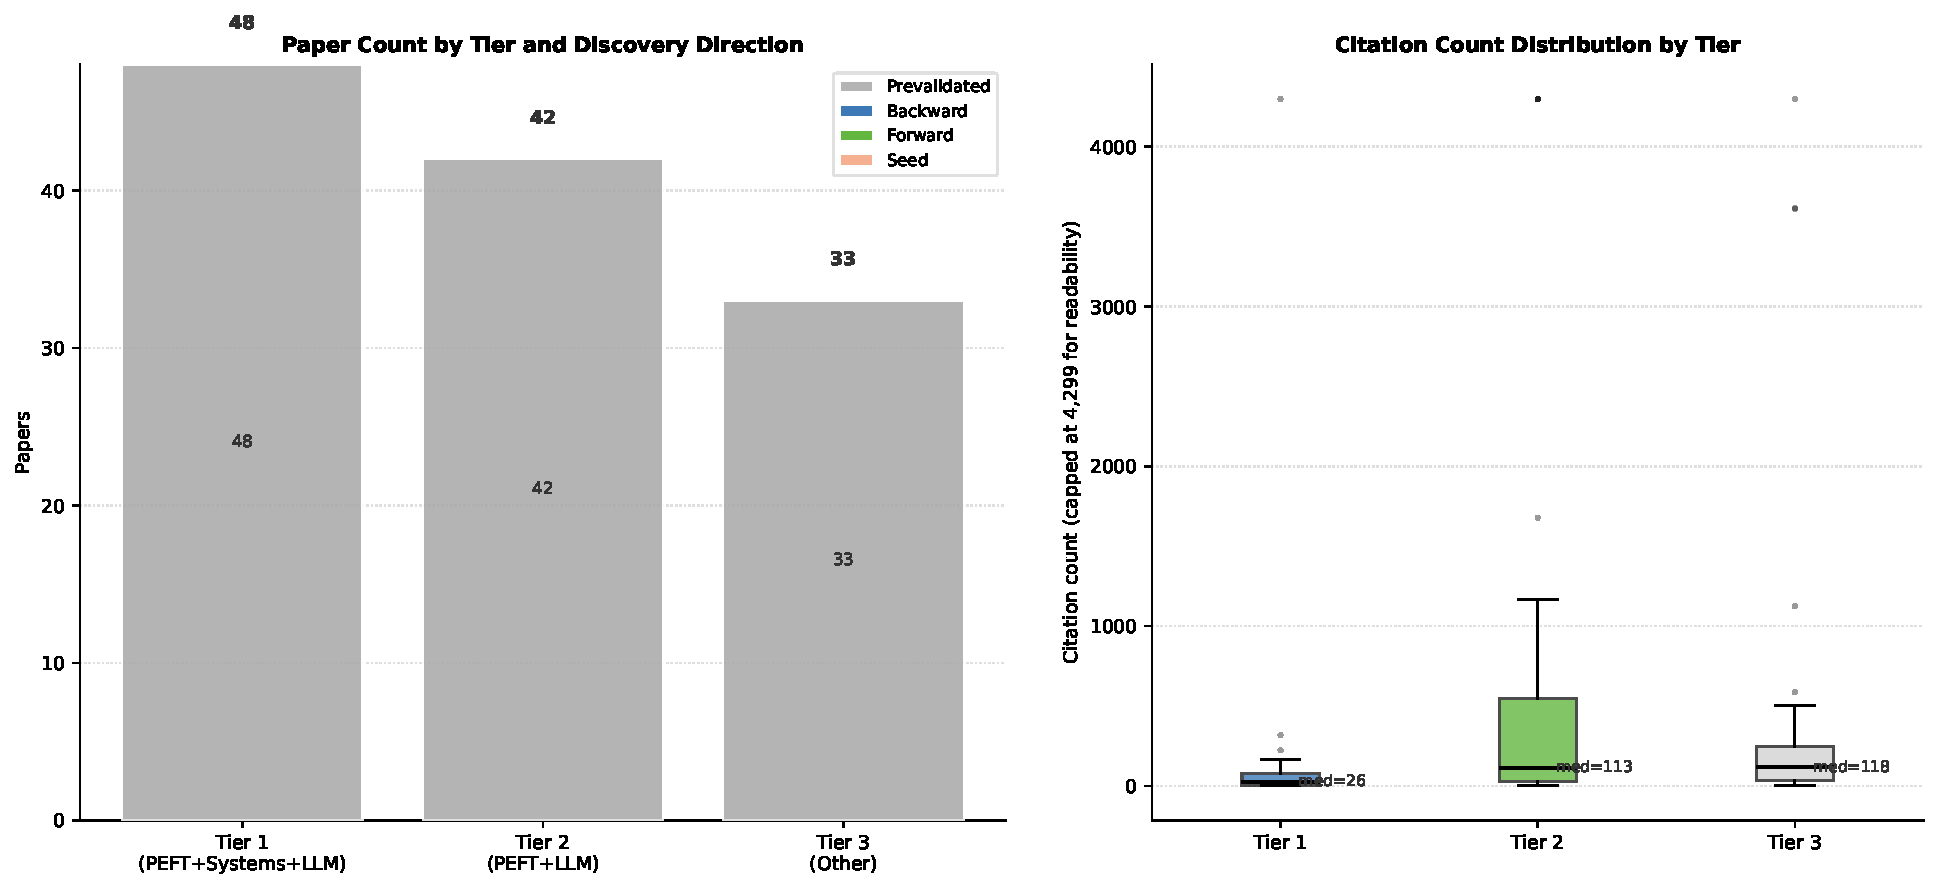
\includegraphics[width=1\linewidth]{figures/fig_slr6_tier_breakdown.pdf}
  \caption{Tier breakdown of the 123-record final list (cf.\ Table~\ref{tab:tiers}
           for the enrichment-stage tiering of the 464-record pool).
           Tier~1 (48, 39.0\%): PEFT + distributed/P2P + LLM (all three);
           Tier~2 (42, 34.1\%): two of the three themes;
           Tier~3 (33, 26.8\%): foundational or tangential (one theme). The right panel shows the
           citation-count distribution by tier for the 123 records.}
  \label{fig:tiers}
\end{figure}

Tiers (Figure~\ref{fig:tiers}) served as a reading-priority guide following the three-pass method of
Keshav~\cite{Keshav2007}: Tier~1 papers received full reads, Tier~2
selective reads, and Tier~3 abstract-level assessment. Venue quality of the
464-paper corpus: 166 papers (35.8\%) were published in a venue ranked
CORE A$^*$ (the top tier of the CORE conference ranking) or in the first
quartile (Q1) of Scopus's journal-impact quartiles; 189 (40.7\%) in other peer-reviewed conferences or journals; 91
(19.6\%) were arXiv preprints without a published venue; and 18 (3.9\%) had
unknown or missing venue metadata.

Table~\ref{tab:extraction_codebook} documents the column schema of the data
extraction table (`\texttt{\seqsplit{11\_data\_extraction\_2026-05-12.csv}}`, 224 rows) that feeds
the funnel in Section~\ref{sec:methodology:search}. Coverage reports the number
of the 224 rows carrying a non-null value. Three schema columns
(`method\_name`, `datasets`, `metrics`) are uniformly empty in the archived
export; the quantitative evaluation evidence they were intended to hold is
instead captured narratively in `key\_finding`/`notes\_raw`, and the
corresponding appraisal dimensions are handled in
Section~\ref{sec:methodology:quality}.

\begin{sidewaystable}[p]
\centering
\caption{Data-extraction codebook: column schema, meaning, allowed values, and
coverage of the 224-row extraction table.}
\label{tab:extraction_codebook}
\small
\setlength{\tabcolsep}{4pt}
  \begin{tabular}{lp{4.5cm}p{5.4cm}r}
\toprule
\textbf{Column} & \textbf{Meaning} & \textbf{Allowed / typical values} & \textbf{Coverage} \\
\midrule
\texttt{paper\_key} & Internal record key (arXiv ID, DOI, or Scopus hash) & arXiv id / DOI / 40-hex Scopus hash & 223/224 \\
\texttt{arxiv\_id} & arXiv identifier, where applicable & \texttt{YYYY.NNNNN} & 81/224 \\
\texttt{doi} & Digital Object Identifier & DOI string & 185/224 \\
\texttt{title} & Article title & free text & 224/224 \\
\texttt{authors} & Author list & semicolon-separated & 217/224 \\
\texttt{year} & Publication year & 4-digit year & 223/224 \\
\texttt{venue} & Publishing venue & venue name & 221/224 \\
\texttt{citation\_count} & Citations at retrieval (from Crossref/SS) & non-negative integer & 205/224 \\
\texttt{tier} & Reading-priority tier & \texttt{1}/\texttt{2}/\texttt{3} (see Table~\ref{tab:tiers}) & 190/224 \\
\texttt{review\_source} & Whether the record proceeded from full-text or abstract second pass & \texttt{fulltext} / \texttt{abstract-2nd-pass} & 190/224 \\
\texttt{corpus} & Relevance position & \texttt{core} / \texttt{background} & 190/224 \\
\texttt{contribution\_type} & Inferred contribution category & one of 15 categories (per-table text) & 190/224 \\
\texttt{peft\_technique} & PEFT technique used & e.g.\ \texttt{LoRA}, \texttt{bottleneck adapter}, \texttt{prefix}, \texttt{generic-PEFT}, \texttt{none} & 190/224 \\
\texttt{distribution\_mechanism} & How model/adapter state is shared & e.g.\ \texttt{federated}, \texttt{P2P/gossip}, \texttt{centralised server}, \texttt{DHT}, \texttt{none} & 190/224 \\
\texttt{thesis\_sections} & Review sections citing the paper & \texttt{\S n.n} references & 190/224 \\
\texttt{contribution\_codes} & Novel-contribution tag(s) & \texttt{\ccstar A1/S1/R1/R2/T2/M2} combinations & 22/224 \\
\texttt{method\_name}, \texttt{datasets}, \texttt{metrics} & Schema columns retained but not populated in the archived extraction & --- & 0/224 \\
\texttt{key\_finding} & One-line primary outcome / contribution summary & free text (max ~1--2 lines) & 190/224 \\
\texttt{notes\_raw} & Full-text reading notes (methods, results, \texttt{\S} and \texttt{\ccstar} tags) & free text & 190/224 \\
\texttt{source} & Retrieval source & \texttt{SCOPUS} / \texttt{ARXIV} / \texttt{WOS} & 220/224 \\
\bottomrule
  \end{tabular}
\end{sidewaystable}

\subsection*{A.6 Bibliometric Overview}

The final corpus of 123 papers spans the period 2002--2026 (Table~\ref{tab:year_dist};
Figure~\ref{fig:bibliometric}), with a marked concentration in
the 2021--2025 window (106 papers, 86\% of the corpus). The most 
active year is 2024 with 38 papers (31\% of total), followed by 
2023 with 20 (16\%) and 2025 with 19 (15\%), confirming that 
the field is both active and growing. Publication volume 
accelerates sharply after 2022, coinciding with the proliferation 
of LoRA-based PEFT papers and adapter-serving systems.

\begin{table}[H]
\centering
\caption{Publication year distribution of the 123-paper reviewed corpus. The
\% column sums to 100.1 due to rounding.}
\label{tab:year_dist}
\begin{tabular}{lrr}
\toprule
\textbf{Year} & \textbf{Papers} & \textbf{\% of corpus} \\
\midrule
2002 & 1 & 0.8 \\
2011 & 1 & 0.8 \\
2016 & 1 & 0.8 \\
2017 & 1 & 0.8 \\
2019 & 4 & 3.3 \\
2020 & 5 & 4.1 \\
2021 & 17 & 13.8 \\
2022 & 12 & 9.8 \\
2023 & 20 & 16.3 \\
2024 & 38 & 30.9 \\
2025 & 19 & 15.4 \\
2026 & 4 & 3.3 \\
\midrule
\textbf{Total} & \textbf{123} & \textbf{100} \\
\bottomrule
\end{tabular}
\end{table}

\begin{figure}[H]
  \centering
  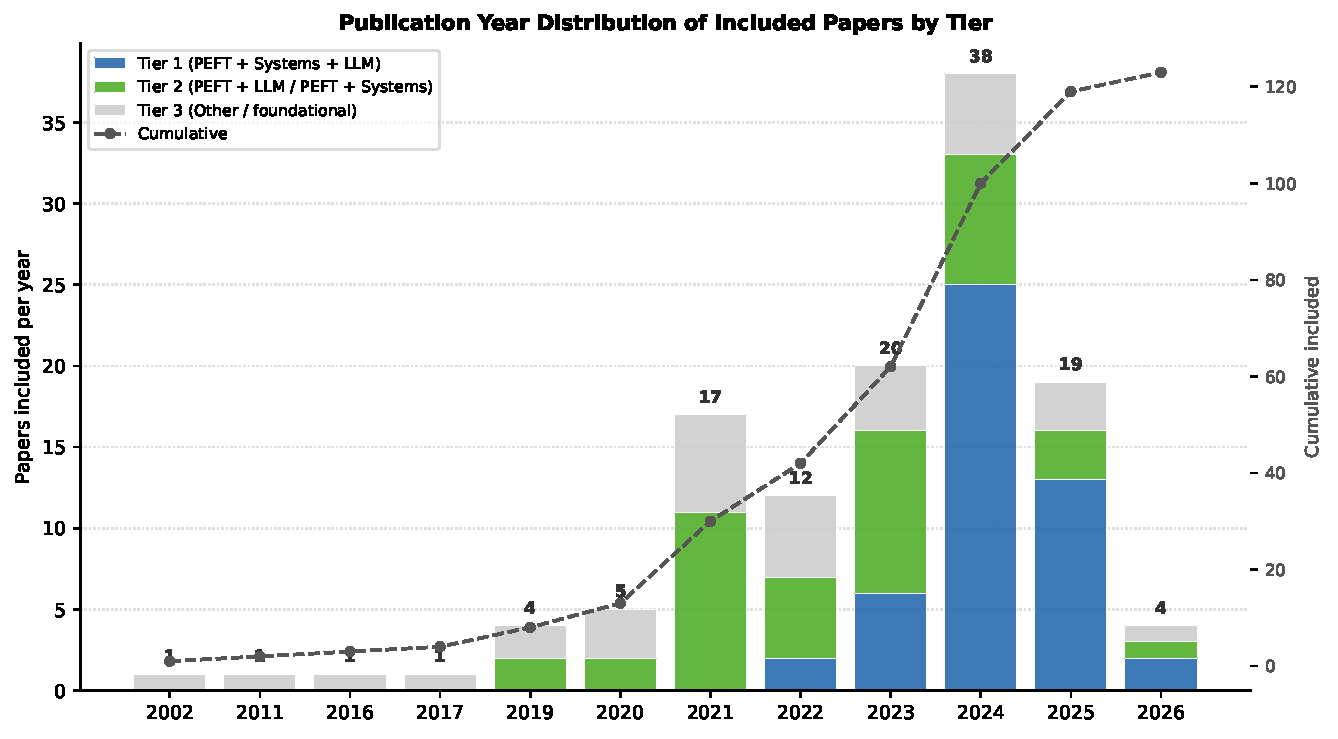
\includegraphics[width=1\linewidth]{figures/fig_slr3_year_distribution.pdf}
  \caption{Year distribution of the 123-paper reviewed corpus,
           showing the acceleration of publication volume from 2023 onward.}
  \label{fig:bibliometric}
\end{figure}

Figure~\ref{fig:venues} reports the venue distribution of the 123-paper
final corpus discussed above (the same population as
Figure~\ref{fig:bibliometric}).

\begin{figure}[H]
  \centering
  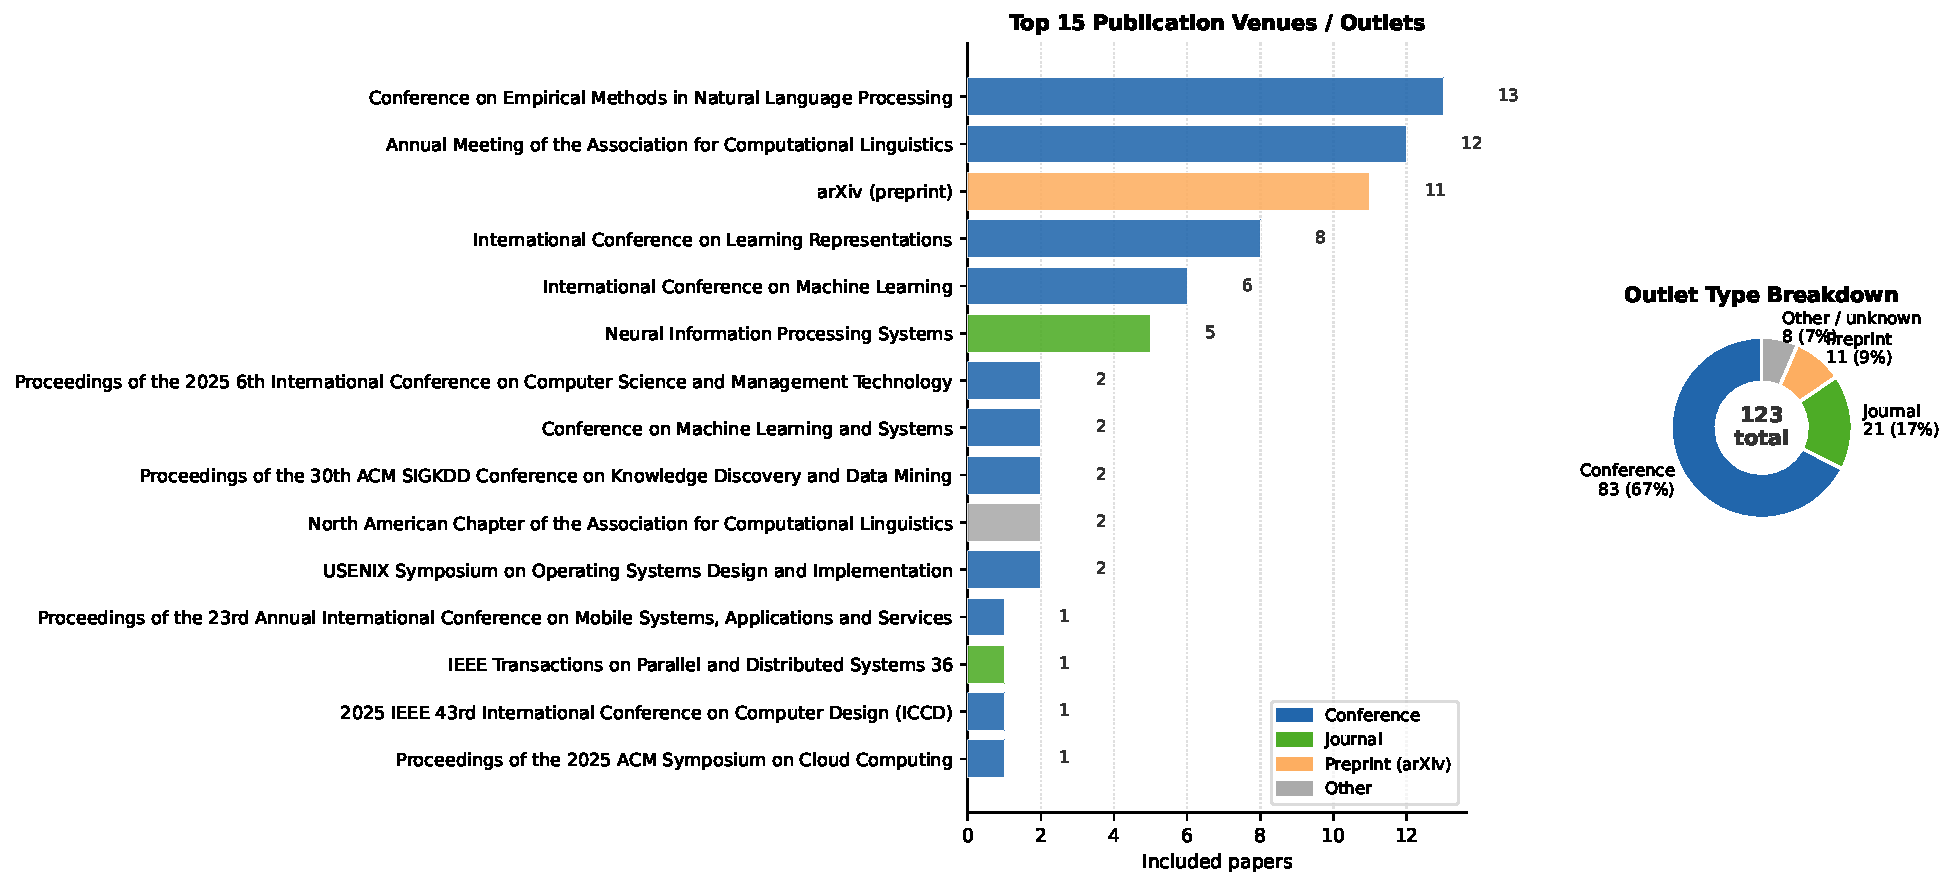
\includegraphics[width=1\linewidth]{figures/fig_slr5_venues.pdf}
  \caption{Venue distribution of the 123-paper final corpus. ACL/EMNLP
           comprises the largest venue category (25 papers), followed by
           arXiv preprints (11), ICLR (8), ICML/MLSys (9), and NeurIPS (5).}
  \label{fig:venues}
\end{figure}

The most densely covered concept-matrix dimension is \textbf{adapter
exchange} (present in the majority of the 123 papers), while
\textbf{peer-to-peer topology} and \textbf{discovery mechanism} remain the
least covered dimensions, directly motivating the gaps identified in
Section~\ref{sec:synthesis_gap}.

\subsection*{A.7 Abstract-Level Review}

Following Keshav~\cite{Keshav2007}, the author conducted an abstract-level
review across all 552 records (464 enriched corpus records --- the 32
deprioritised low-citation arXiv preprints in the rescue file were confirmed
excluded and were not reinstated --- plus 88 records from forward citation
snowballing on Scopus and WoS that were title-screened and added to the
review). To support decision
consistency across a corpus of this size, each abstract was accompanied by an
automated advisory note --- produced by Claude Sonnet (Anthropic,
\texttt{claude-sonnet-4-6}) --- providing a one-sentence summary, a relevance
assessment relative to the three core themes, and a preliminary KEEP / SKIP /
DEFER recommendation. These notes served as a consistency aid; all final
decisions were made by the author after independent assessment. The
resulting disposition of the 552-record pool is reported in
Table~\ref{tab:abstract}. The advisory notes were shown in the interactive
screener and not separately exported; the author's final KEEP / SKIP / DEFER
decision is logged per record (column \texttt{abstract\_decision}) in
\texttt{S7b\_abstract\_reviewed\_final.csv} to support reproducibility checks.

\begin{table}[H]
\centering
\caption{Abstract-review disposition of the 552-record pool, matching
Figure~\ref{fig:prisma}. The three-way KEEP / DEFER / SKIP split is the
canonical classification. DEFER records were not disposed of as SKIP: they
were carried into the full-text review queue (214 KEEP ${}+{}$ 173 DEFER =
387 queued; see text), and a subset was read in full before being excluded
at final curation — none reached the data-extraction stage.}
\label{tab:abstract}
\begin{tabular}{lrr}
\toprule
\textbf{Decision} & \textbf{\textit{N}} & \textbf{\%} \\
\midrule
KEEP (exported to the full-text review queue)          & 214 & 38.8 \\
DEFER (re-flagged for closer inspection; also queued)  & 173 & 31.3 \\
SKIP (excluded at abstract review, did not proceed)    & 165 & 29.9 \\
\midrule
\textbf{Total reviewed}                                & \textbf{552} & \\
\bottomrule
\end{tabular}
\end{table}

\emph{Derived rollup (for reference, KEEP vs.\ combined DEFER${}+{}$SKIP).}
Collapsing DEFER into the not-advanced group gives a two-way view of
\textbf{214} KEEP (38.8\%) and \textbf{338} not advanced immediately
(61.2\%); this is a presentational rollup of the canonical three-way
classification above and \emph{not} an alternative final count, since the
173 DEFER records were carried into the 387-record full-text queue.

KEEP papers were exported for full-text review via RIS format
(\texttt{\seqsplit{08\_zotero\_ready\_2026-05-02.ris}}, 214 entries). The full-text
review queue (\texttt{\seqsplit{09\_fulltext\_review\_queue\_2026-05-02.csv}}),
compiled from the 214 KEEP and the 173 borderline-DEFER records, contains
\textbf{387} records; of these, \textbf{190} proceeded to data extraction (all
KEEP-origin; no DEFER-origin records reached extraction) and \textbf{197} were
excluded (24 KEEP-origin, full text unavailable; 173 DEFER-origin, not taken
further). A
separate manual Scopus/WoS cross-validation top-up of \textbf{34} records
entered directly at the extraction stage, bypassing this full-text queue
(none were ultimately retained in the final 123), bringing the extraction
set to \textbf{224} (\texttt{\seqsplit{11\_data\_extraction\_2026-05-12.csv}}). A subset of the
queued DEFER records was read in full during this phase but was excluded at
the final curation step (Supplementary Material S4, \S~D).
Every record and its per-stage membership are traceable in the unified
pipeline file (\texttt{\seqsplit{pipeline\_unified.csv}}). The final reading list
(\texttt{\seqsplit{13\_final\_reading\_list\_2026-05-12.csv}}) is the authoritative
evidentiary base: \textbf{only the 123 papers it lists} entered the final
inclusion set for this review. Records from earlier pipeline stages whose full
text was not obtained (whether marked \texttt{DEFER} or left un-assessed, and
in each case because no PDF was downloaded) were not included in the final
reading list. The evidence presented in this review therefore rests solely on
these 123 papers.

